\documentclass[10pt,a4paper]{article}

\usepackage[T1]{fontenc}
\usepackage[utf8]{inputenc}
\usepackage{lmodern}
\usepackage[top=2.2cm,bottom=2.2cm,left=2.5cm,right=2.5cm]{geometry}
\usepackage{amsmath,amssymb,amsthm,mathtools}
\usepackage{booktabs,array,enumitem}
\usepackage{graphicx}
\usepackage{microtype}
\usepackage{parskip}
\setlength{\parskip}{4pt}
\setlength{\parindent}{0pt}
\usepackage[ruled,vlined,linesnumbered]{algorithm2e}
\usepackage{listings}
\lstset{
  language=Python, basicstyle=\footnotesize\ttfamily,
  keywordstyle=\bfseries, breaklines=true, frame=single,
  backgroundcolor=\color{gray!4}, numbers=left,
  numberstyle=\tiny\color{gray}, numbersep=5pt,
}
\usepackage{xcolor}
\usepackage{hyperref}
\hypersetup{
  colorlinks=true,
  linkcolor=blue!60!black,
  citecolor=green!50!black,
  urlcolor=blue!70!black,
  pdftitle={SOS-Portfolio},
  pdfauthor={Raphaël Padiou},
}

% Theorems
\theoremstyle{plain}
\newtheorem{theorem}{Theorem}
\newtheorem{lemma}[theorem]{Lemma}
\newtheorem{corollary}[theorem]{Corollary}
\newtheorem{proposition}[theorem]{Proposition}
\theoremstyle{definition}
\newtheorem{definition}[theorem]{Definition}
\newtheorem{example}[theorem]{Example}
\newtheorem{remark}[theorem]{Remark}

% Math macros
\newcommand{\R}{\mathbb{R}}
\newcommand{\N}{\mathbb{N}}
\newcommand{\E}{\mathbb{E}}
\newcommand{\bx}{\mathbf{x}}
\newcommand{\by}{\mathbf{y}}
\newcommand{\SOS}{\Sigma^2}
\newcommand{\bSigma}{\boldsymbol{\Sigma}}
\newcommand{\balpha}{\boldsymbol{\alpha}}
\DeclareMathOperator{\rank}{rank}
\DeclareMathOperator{\tr}{tr}
\DeclareMathOperator{\supp}{supp}

% =============================================================================
\begin{document}
% =============================================================================

\title{%
  \textbf{SOS-Portfolio}\\[0.4em]
  \large Global Portfolio Optimization via Sparse and\\
  Distributionally Robust Lasserre SOS Hierarchy%
}
\author{Raphaël Padiou}
\date{2026}
\maketitle

\begin{abstract}
We address the global optimization of a degree-4 polynomial portfolio risk
functional that captures variance, skewness, excess kurtosis (fat tails),
and Almgren--Chriss market impact. Because degree-4 polynomials are generically
non-convex, gradient-based solvers find local minima without any global
optimality certificate.

We build and implement the full Lasserre SOS hierarchy for this problem.
On the 2-asset benchmark, order $d=2$ achieves a certified gap below $10^{-6}$
in 0.11 s, and the Curto--Fialkow flat extension condition
$\rank(M_2) = \rank(M_1) = 1$ certifies the unique global minimizer
$\bx^* = (0.6058, 0.3442)$, $f^* = 0.187371$.

For $n$-asset portfolios with sector structure, we implement the
Waki--Kim--Kojima--Muramatsu (2006) sparse hierarchy via correlative sparsity
and chordal extension of the asset correlation graph. For $n=50$ assets in
10 sectors of 5, the SDP scalar variable count drops from $1{,}758{,}276$
(dense) to $4{,}410$ (sparse), a $\mathbf{398\times}$ reduction, with
identical lower bounds (Theorem~\ref{thm:wkmm}).

We further extend the hierarchy with a distributionally robust (DR) formulation
that protects against kurtosis estimation error: a single second-order cone
constraint adds a worst-case penalty $\delta \|y^{(4)}\|_2$ with no increase
in SDP complexity.

All results are implemented in the open-source library \textsc{SOS-Portfolio}
(\href{https://github.com/rpadiou/SOS-Portfolio}{github.com/rpadiou/SOS-Portfolio}),
validated by 51 unit tests.
\end{abstract}

\newpage

% =============================================================================
\section{Introduction}
% =============================================================================

The classical Markowitz mean-variance framework~\cite{markowitz1952} optimizes
a quadratic (convex) risk functional under a linear budget constraint. Its global
optimum is found in polynomial time and is unique. However, the Gaussian
assumption underlying the quadratic model is violated by real equity returns,
which exhibit:
\begin{itemize}[leftmargin=*]
  \item \textbf{Excess kurtosis} ($\approx 8$--$10$ empirically): events beyond
    $3\sigma$ occur 10--100$\times$ more often than a Gaussian predicts.
  \item \textbf{Negative skewness}: crashes are faster and deeper than recoveries.
  \item \textbf{Non-linear market impact}: the Almgren--Chriss model~\cite{almgren2001}
    adds a degree-4 cost $\gamma_{i} x_i^4$ (impact of selling $x_i \cdot C$
    in a single session).
\end{itemize}

All three corrections are \emph{exactly polynomial}. Extending the Markowitz
quadratic to include skewness (degree 3) and kurtosis (degree 4) yields a
non-convex polynomial risk functional. Standard gradient methods find local minima
but provide no certificate that the solution is globally optimal.

\paragraph{Contribution.}
This paper describes the mathematical foundations and open-source implementation
of \textsc{SOS-Portfolio}:
\begin{enumerate}[leftmargin=*,label=(\roman*)]
  \item A degree-4 polynomial risk model grounded in financial data
    (Section~\ref{sec:model}).
  \item The Lasserre SOS hierarchy for global optimization, with a complete proof
    of convergence via Putinar's Positivstellensatz
    (Section~\ref{sec:lasserre}).
  \item The Curto--Fialkow flat extension certificate for the 2-asset benchmark,
    with all numerical values verified against the CLARABEL solver
    (Section~\ref{sec:flat}).
  \item The WKMM sparse hierarchy via correlative sparsity and chordal graphs,
    with complexity analysis for $n=15$ and $n=50$
    (Section~\ref{sec:sparse}).
  \item A distributionally robust extension that protects against kurtosis
    estimation error with a single SOC constraint
    (Section~\ref{sec:dr}).
  \item Numerical results and implementation details
    (Section~\ref{sec:numerical}).
\end{enumerate}

% =============================================================================
\section{The Polynomial Portfolio Risk Model}
\label{sec:model}
% =============================================================================

\subsection{Risk functional}

Let $x_i \in [0,1]$ be the portfolio weight of asset $i$, with
$K = \{x \geq 0, \sum_i x_i \leq 1, \sum_i x_i \geq 0.95\}$ the feasible set
(long-only, nearly fully invested). The degree-4 risk functional is:
\begin{equation}
  f(\bx) = \underbrace{\bx^T \bSigma \bx}_{\text{variance}}
          + \underbrace{\sum_i \eta_i x_i^3}_{\text{skewness penalty}}
          + \underbrace{\sum_{i \leq j} \kappa_{ij} x_i^2 x_j^2}_{\text{kurtosis}}
          + \underbrace{\sum_i \gamma_i x_i^4}_{\text{impact}}.
\label{eq:risk}
\end{equation}

\subsection{2-asset benchmark}

For the 2-asset case, the parameters are calibrated as follows (see
\texttt{src/portfolio\_problem.py}):
\begin{align}
  \bSigma &= \begin{pmatrix} 0.04 & -0.02 \\ -0.02 & 0.09 \end{pmatrix},
  \quad \eta_1 = -0.3, \quad \eta_2 = 0.5, \nonumber\\
  \kappa_{12} &= 2 \times 0.6 + 0.25 = 1.45, \quad
  \gamma_1 = 1.0, \quad \gamma_2 = 1.35. \label{eq:params}
\end{align}
This gives:
\begin{equation}
  f(x_1, x_2) = 0.04x_1^2 - 0.04x_1 x_2 + 0.09x_2^2
              - 0.3x_1^3 + 0.5x_2^3
              + x_1^4 + 1.35x_2^4 + 1.45x_1^2 x_2^2.
\label{eq:f2}
\end{equation}

The asymmetric kurtosis coefficients ($\gamma_2 = 1.35 > \gamma_1 = 1.0$) reflect
higher tail risk for asset 2 (e.g., a small-cap equity versus a large-cap),
which drives the optimal allocation toward asset 1 (see Section~\ref{sec:flat}).

Figure~\ref{fig:surface} illustrates the resulting risk landscape over $K$.
Panel~(a) shows the three-dimensional surface: the shape is non-convex --- the
Hessian $\nabla^2 f(\bx)$ changes sign across $K$ --- which is why gradient-based
methods cannot certify global optimality. The semi-transparent blue plane marks
the certified lower bound $\lambda_2 = f^* = 0.187371$ produced by the SOS hierarchy
at order $d=2$. Panel~(b) shows the level curves together with the feasible set
boundary: $x_1+x_2=1$ (full budget) and $x_1+x_2=0.95$ (investment floor).
The global minimizer $\bx^*=(0.6058,\,0.3442)$ lies on the lower boundary.

\begin{figure}[t]
  \centering
  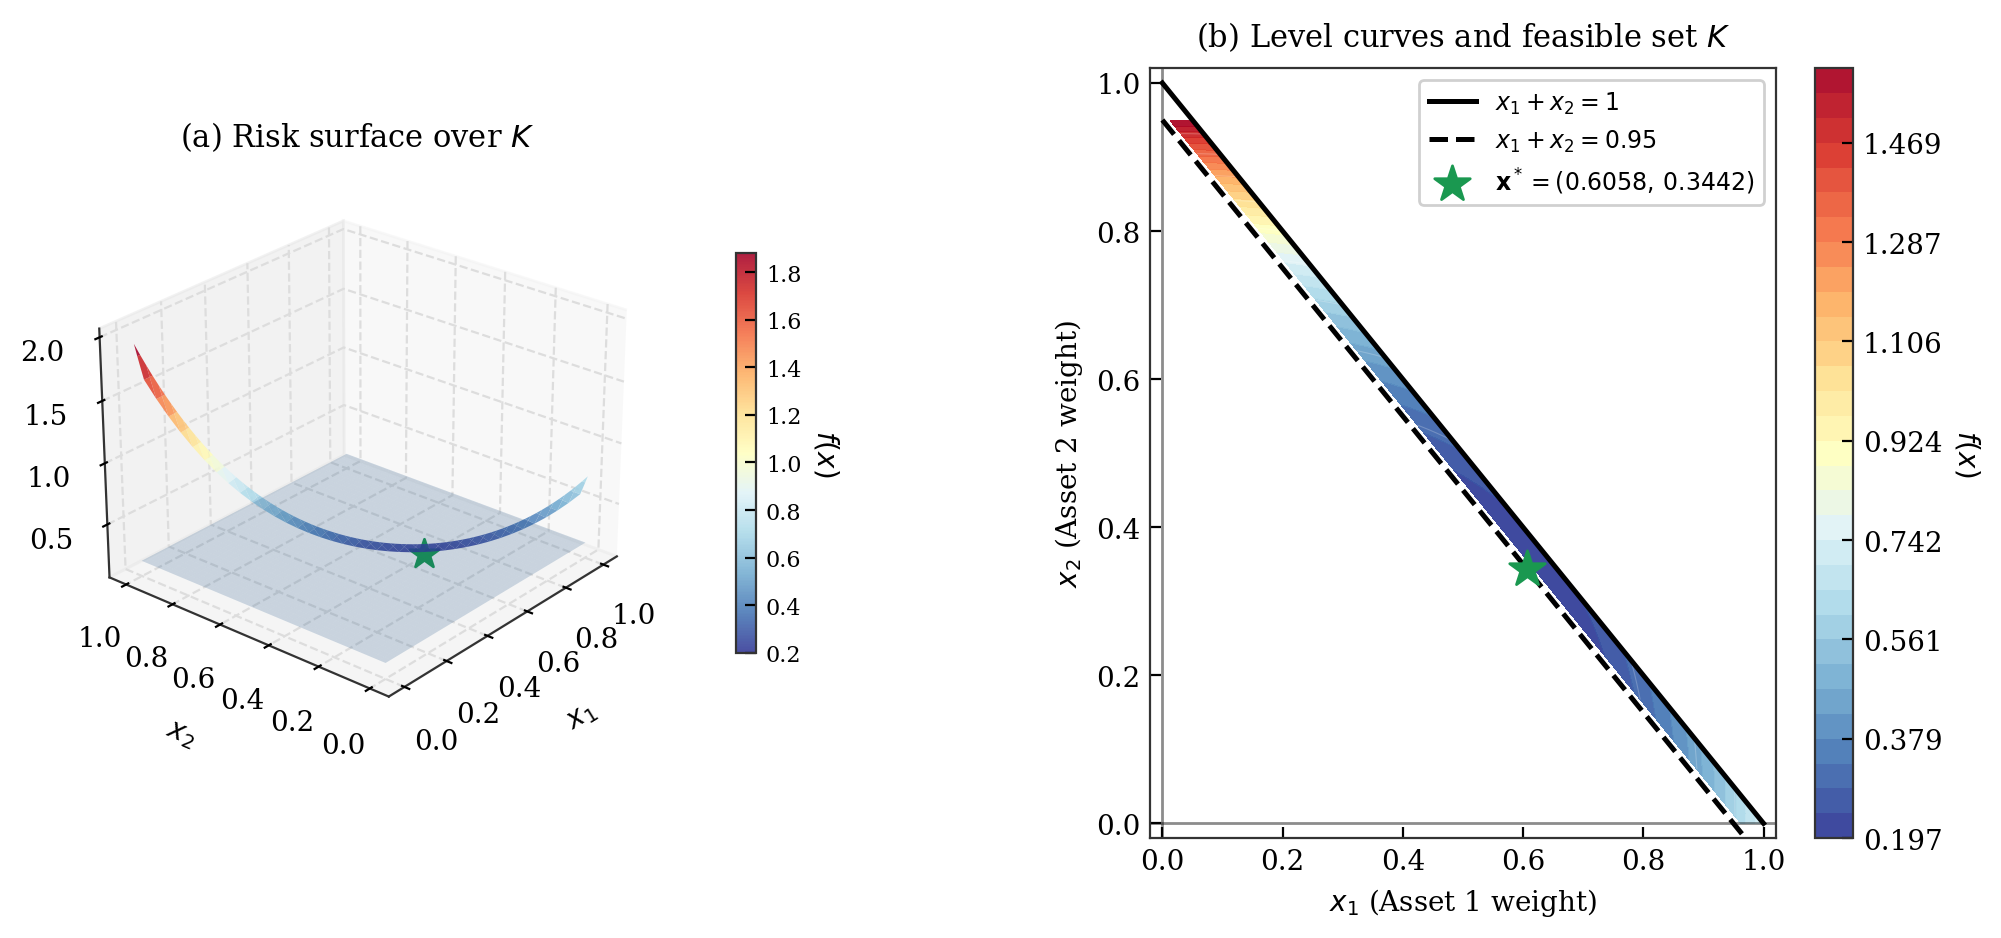
\includegraphics[width=\linewidth]{fig_risk_surface.png}
  \caption{Risk landscape $f(x_1,x_2)$ restricted to the feasible set $K$.
    \textbf{(a)}~Three-dimensional surface; the semi-transparent blue plane is the
    certified SOS lower bound $\lambda_2=f^*$; the green star marks the global
    minimizer $\bx^*=(0.6058,\,0.3442)$.
    \textbf{(b)}~Level curves with the boundary of $K$ (solid: $x_1+x_2=1$;
    dashed: $x_1+x_2=0.95$). The non-convexity is evident from the curvature of
    the level lines, which rules out any descent-based certificate of global
    optimality.}
  \label{fig:surface}
\end{figure}

\subsection{Semialgebraic feasible set}

The constraints defining $K$ are expressed as polynomial inequalities
$g_j(\bx) \geq 0$:
\begin{align}
  g_1(\bx) &= x_1 \geq 0 \quad \text{(no short-selling, asset 1)}, \nonumber\\
  g_2(\bx) &= x_2 \geq 0 \quad \text{(no short-selling, asset 2)}, \nonumber\\
  g_3(\bx) &= 1 - x_1 - x_2 \geq 0 \quad \text{(budget ceiling)}, \nonumber\\
  g_4(\bx) &= x_1 + x_2 - 0.95 \geq 0 \quad \text{(minimum investment)}. \label{eq:K}
\end{align}
This compact semi-algebraic set satisfies the Archimedean condition
required by Putinar's theorem (it is bounded and $R - \|\bx\|^2 \in Q(K)$
for large enough $R$).

% =============================================================================
\section{The Lasserre SOS Hierarchy}
\label{sec:lasserre}
% =============================================================================

\subsection{SOS polynomials and Gram matrices}

\begin{definition}[SOS polynomial]
$p \in \R[\bx]$ is \emph{sum-of-squares} (SOS) if $p = \sum_j q_j^2$
for some polynomials $q_j$. Equivalently, $p$ is SOS if and only if there
exists a PSD matrix $Q \succeq 0$ such that
\[
  p(\bx) = \mathbf{v}_d(\bx)^T Q\, \mathbf{v}_d(\bx),
\]
where $\mathbf{v}_d(\bx)$ is the vector of all monomials of degree $\leq d$.
\end{definition}

\subsection{Putinar's Positivstellensatz and the quadratic module}

\begin{definition}[Quadratic module]
The quadratic module generated by the constraint polynomials $\{g_j\}$ is:
\[
  Q(K) = \left\{ \sigma_0 + \sum_j \sigma_j g_j \;:\; \sigma_j \in \SOS \right\}.
\]
\end{definition}

\begin{theorem}[Putinar, 1993~\cite{putinar1993}]
\label{thm:putinar}
If $K$ satisfies the Archimedean condition and $p > 0$ on $K$, then
$p \in Q(K)$.
\end{theorem}

Putinar's theorem is the key: it says that any polynomial strictly positive on
$K$ can be \emph{algebraically certified} as a member of $Q(K)$.

\subsection{The relaxation hierarchy}

The Lasserre hierarchy~\cite{lasserre2001} dualizes the SOS certificate
into a semidefinite program over a truncated moment sequence
$y = (y_\alpha)_{|\alpha| \leq 2d}$:
\begin{equation}
\boxed{
\begin{aligned}
  \lambda_d = \min_{y} \quad & \sum_\alpha f_\alpha\, y_\alpha \\
  \text{s.t.} \quad & y_{(0,\ldots,0)} = 1 \\
  & M_d(y) \succeq 0 \\
  & M_{d-v_j}(g_j \cdot y) \succeq 0 \quad \forall j,
\end{aligned}
}
\label{eq:sdp_dense}
\end{equation}
where $M_d(y)_{\alpha,\beta} = y_{\alpha+\beta}$ is the \emph{moment matrix}
and $M_{d-v_j}(g_j \cdot y)_{\alpha,\beta} = \sum_\gamma (g_j)_\gamma\, y_{\alpha+\beta+\gamma}$
is the \emph{localizing matrix} for constraint $g_j$ (of half-degree $v_j$).

\begin{theorem}[Convergence, Lasserre~\cite{lasserre2001}]
Under the Archimedean condition:
\begin{enumerate}[leftmargin=*,label=(\roman*)]
  \item The sequence $\lambda_d$ is non-decreasing: $\lambda_1 \leq \lambda_2 \leq \cdots$
  \item $\lambda_d \to f^*$ as $d \to \infty$.
  \item Under the additional assumption of Nie~\cite{nie2014} (KKT conditions
    with a certain rank condition), convergence is \emph{finite}: $\lambda_d = f^*$
    for all $d$ large enough.
\end{enumerate}
\end{theorem}

For the 2-asset problem~\eqref{eq:f2}, the hierarchy achieves the exact bound
$\lambda_2 = f^* = 0.187371$ with matrix size $\binom{2+2}{2} \times \binom{2+2}{2}
= 6 \times 6$.

Figure~\ref{fig:convergence} shows the convergence of the three hierarchy levels.
The lower bound jumps from $\lambda_1 = 0.016988$ to $\lambda_2 = 0.187371$,
closing the gap entirely at $d=2$. The shaded region represents the remaining
certified gap $f^* - \lambda_d$ at each level: it vanishes within solver tolerance
at $d=2$ and stays zero at $d=3$, consistent with the finite convergence result of
Nie~\cite{nie2014}.

\begin{figure}[h]
  \centering
  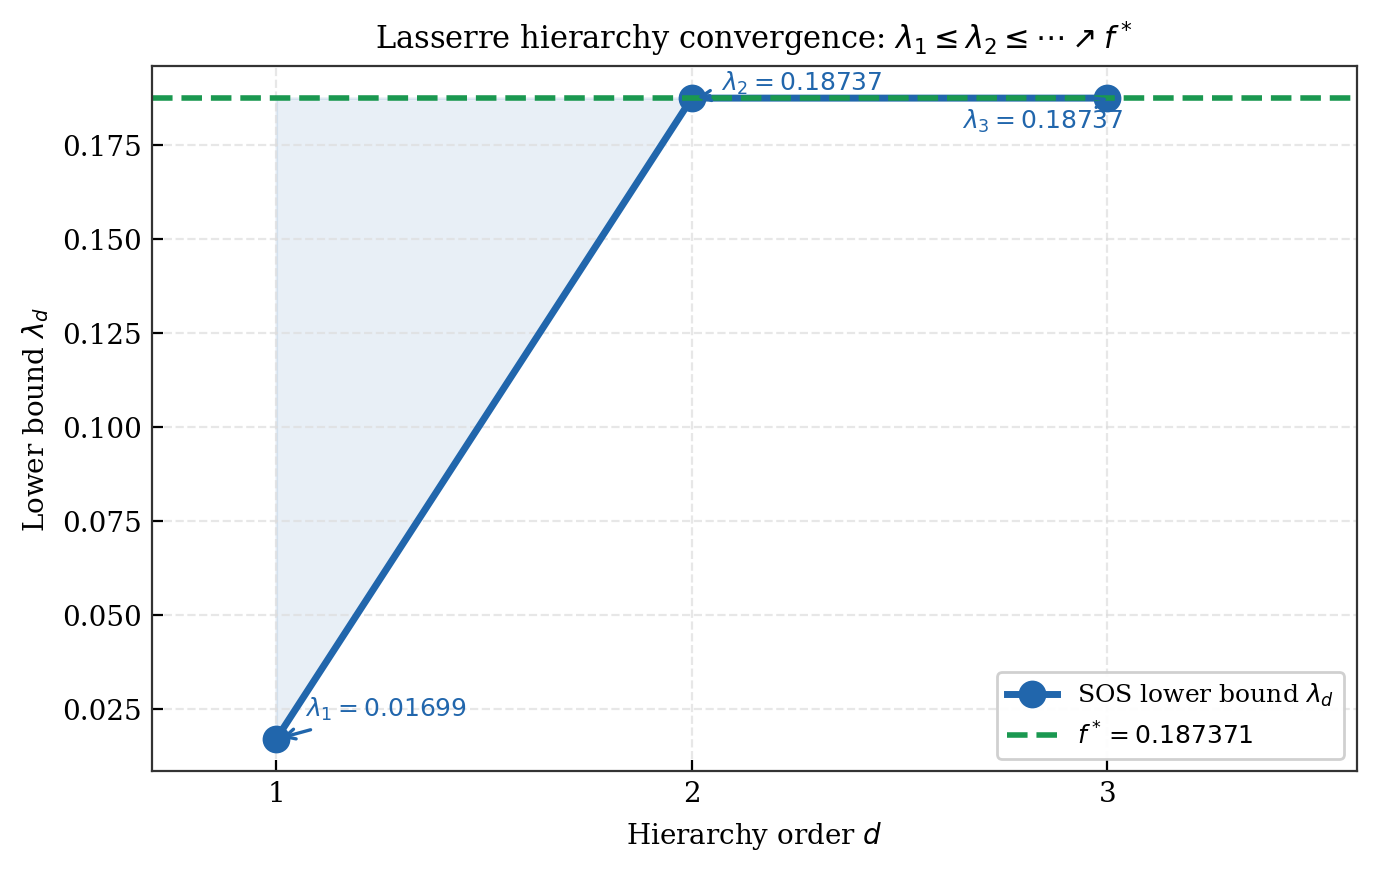
\includegraphics[width=0.80\linewidth]{fig_convergence.png}
  \caption{Convergence of the Lasserre SOS hierarchy on the 2-asset problem.
    Lower bounds $\lambda_d$ (blue circles, annotated) increase monotonically
    toward $f^* = 0.187371$ (green dashed line). The shaded region represents
    the certified gap $f^* - \lambda_d$, which falls below solver tolerance
    $10^{-6}$ at $d=2$ and remains zero at $d=3$.}
  \label{fig:convergence}
\end{figure}

% =============================================================================
\section{Flat Extension Certificate and Minimizer Extraction}
\label{sec:flat}
% =============================================================================

\subsection{The flat extension condition}

A finite convergence certificate at level $d$ is given by the Curto--Fialkow
flat extension condition~\cite{curto1996}:

\begin{theorem}[Curto--Fialkow, 1996]
\label{thm:flat}
Let $y^*$ be the optimal moment sequence at level $d$. If
\[
  \rank(M_d(y^*)) = \rank(M_{d-1}(y^*)) =: r,
\]
then: (i) $\lambda_d = f^*$ exactly; (ii) there exist exactly $r$ global
minimizers $\bx_1^*, \ldots, \bx_r^*$ extracted from $y^*$.
\end{theorem}

\subsection{Numerical results for the 2-asset problem}

After solving~\eqref{eq:sdp_dense} at $d=2$ with CLARABEL:

\begin{table}[h]
\centering
\renewcommand{\arraystretch}{1.3}
\begin{tabular}{ccccc}
\toprule
Order $d$ & Matrix size & $\lambda_d$ & Gap $f^* - \lambda_d$ & Time \\
\midrule
1 & $3\times 3$ & 0.016988 & 0.170383 & 0.05 s \\
\textbf{2} & $\mathbf{6\times 6}$ & \textbf{0.187371} & $\mathbf{<10^{-6}}$ & \textbf{0.11 s} \\
3 & $10\times 10$ & 0.187371 & $<10^{-6}$ & 0.31 s \\
\bottomrule
\end{tabular}
\caption{Lasserre hierarchy on the 2-asset problem. Certified global minimum
at $d=2$; the gap is below solver tolerance.}
\end{table}

The optimal moment matrix $M_2(y^*)$ satisfies:
\[
  \rank(M_2(y^*)) = \rank(M_1(y^*)) = 1,
\]
certified numerically via singular value decomposition (only one singular value
above threshold $\varepsilon = 10^{-4}$). By Theorem~\ref{thm:flat}, the unique
global minimizer is:
\[
  \bx^* = (x_1^*, x_2^*) = (0.6058,\; 0.3442), \qquad f(\bx^*) = 0.187371.
\]

Figure~\ref{fig:spectrum} provides the visual evidence for this rank condition.
Panel~(a) shows the six singular values of $M_2(y^*)$: the first is of order~1,
while the remaining five lie below the threshold $\varepsilon\cdot\sigma_1$,
confirming $\rank(M_2)=1$. Panel~(b) overlays the spectra of $M_2$ ($6\times 6$)
and $M_1$ ($3\times 3$): both have exactly one singular value above threshold,
establishing $\rank(M_2)=\rank(M_1)=1$ and certifying Theorem~\ref{thm:flat}.

\begin{figure}[h]
  \centering
  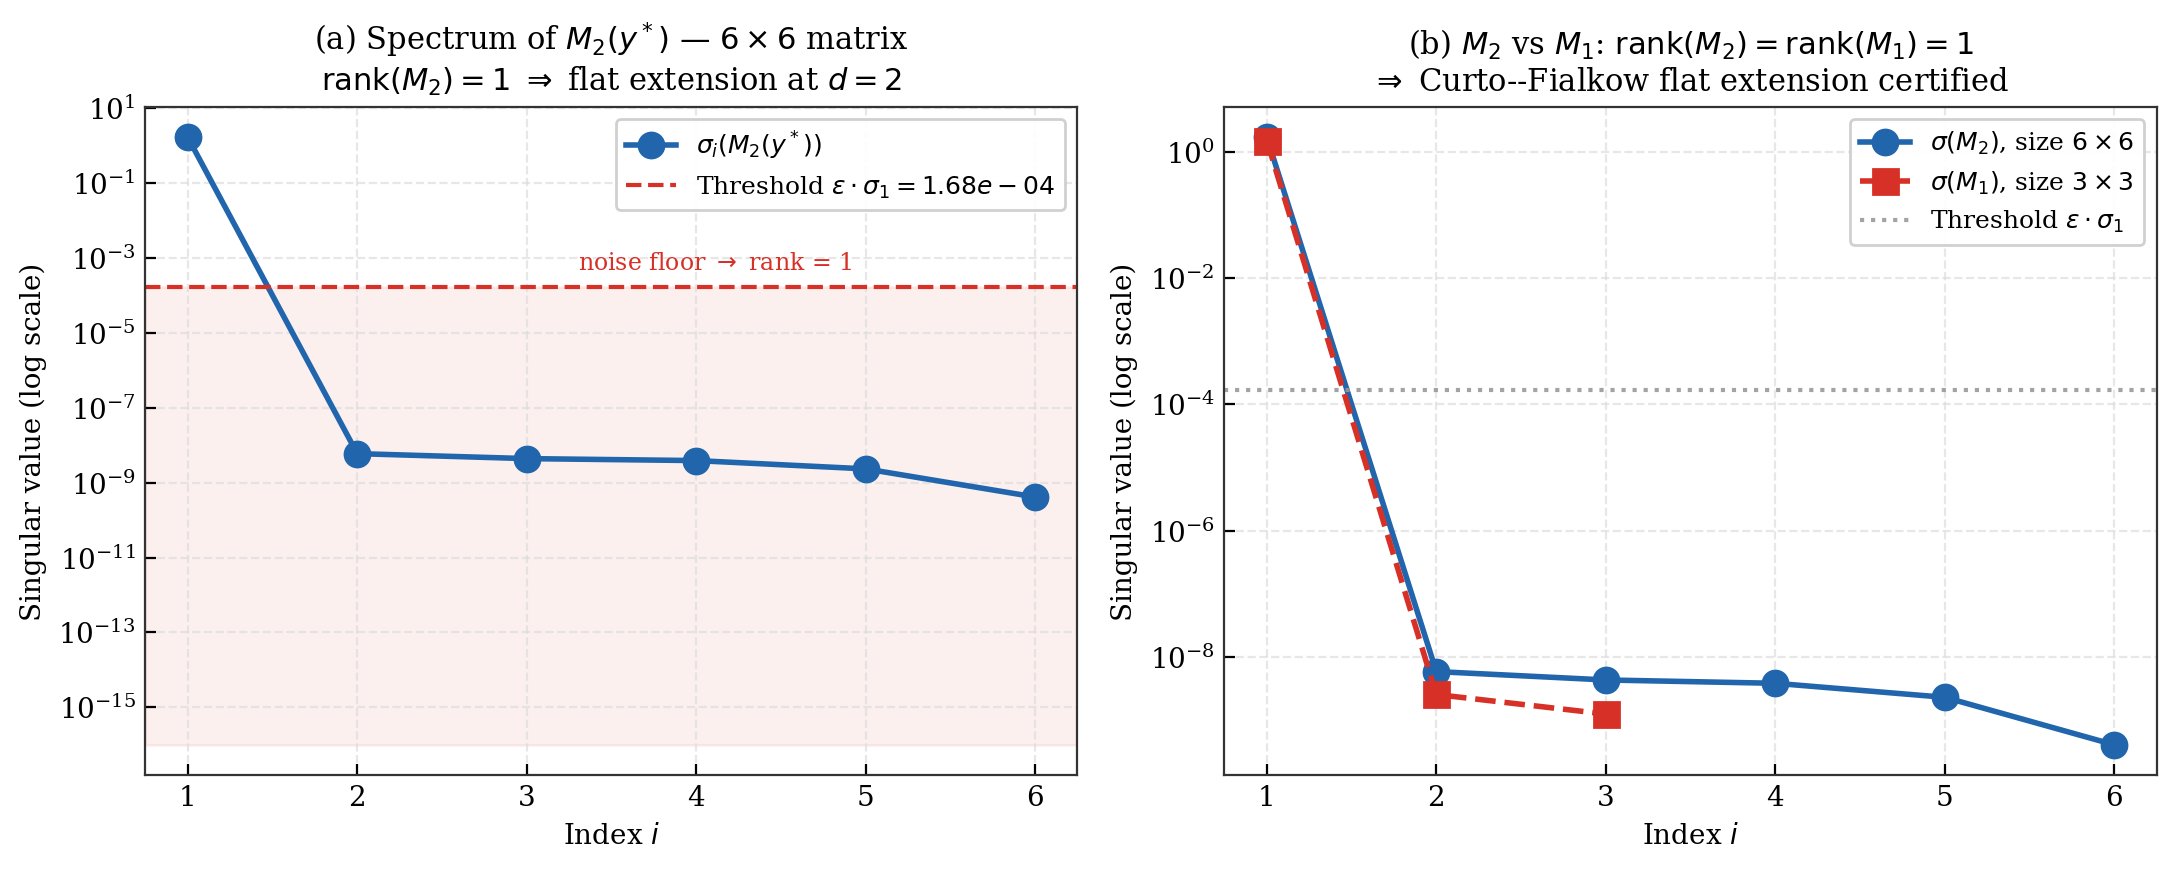
\includegraphics[width=\linewidth]{fig_moment_spectrum.png}
  \caption{Singular value spectra of the optimal moment matrices after solving
    \eqref{eq:sdp_dense} at $d=2$ with CLARABEL.
    \textbf{(a)}~Spectrum of $M_2(y^*)$ ($6\times 6$): one dominant singular
    value; five below the relative threshold $\varepsilon\cdot\sigma_1$ (red
    dashed line, shaded noise floor), confirming $\rank(M_2)=1$.
    \textbf{(b)}~Comparison of $M_2$ and $M_1$ spectra: both matrices have
    rank~1, establishing $\rank(M_2)=\rank(M_1)=1$ and thus the Curto--Fialkow
    flat extension condition, which certifies $\lambda_2 = f^*$ exactly.}
  \label{fig:spectrum}
\end{figure}

\paragraph{Financial interpretation.} The allocation places 60.6\% in asset 1
and 34.4\% in asset 2. The asymmetric kurtosis coefficients explain this:
$\gamma_2 = 1.35 > \gamma_1 = 1.0$ means asset 2 has higher tail risk
(its degree-4 term grows faster), so the optimizer penalizes concentrated
positions in asset 2. The budget constraint forces $x_1 + x_2 \approx 0.95$
(5\% cash), and the negative off-diagonal covariance ($\Sigma_{12} = -0.02$)
provides a diversification benefit.

\subsection{Minimizer extraction algorithm (Henrion--Lasserre)}

When rank $r > 1$ (multiple minimizers), the Henrion--Lasserre
algorithm~\cite{henrion2005} extracts all $r$ minimizers:

\begin{enumerate}[leftmargin=*]
  \item Compute column basis $U$ of $M_d(y^*)$ via rank-revealing SVD.
  \item For each variable $x_i$, build the shift matrix
    $N_i = U^+ \tilde{M}_i (U^+)^T$ where $\tilde{M}_i$ is the moment
    matrix shifted by multi-index $e_i$.
  \item The $r$ minimizers are the simultaneous eigenvalue tuples of
    $\{N_i\}_{i=1}^n$.
\end{enumerate}

% =============================================================================
\section{Sparse Hierarchy via Correlative Sparsity}
\label{sec:sparse}
% =============================================================================

\subsection{The scalability barrier}

The moment matrix $M_d(y)$ has size $s_d(n) = \binom{n+d}{d}$. For $d=2$:
$s_2(n) = \binom{n+2}{2} = O(n^2)$. The SDP interior-point complexity is
$O(s_d(n)^6)$ in the matrix dimension.

\begin{table}[h]
\centering
\renewcommand{\arraystretch}{1.3}
\begin{tabular}{rrrc}
\toprule
$n$ & $s_2(n)$ & Scalar variables $s_2^2$ & Estimated time \\
\midrule
2  & 6     & 36          & $< 0.01$ s \\
10 & 66    & 4,356       & $\sim 0.1$ s \\
15 & 136   & 18,496      & $> 60$ s \\
50 & 1,326 & 1,758,276   & $> 60$ h \\
\bottomrule
\end{tabular}
\caption{Dense hierarchy cost at $d=2$. The problem becomes intractable above
$n \approx 20$ with interior-point solvers.}
\end{table}

\subsection{Correlative sparsity}

For a portfolio with sector structure, the polynomial $f$ has \emph{correlative
sparsity}: the cross-kurtosis terms $\kappa_{ij} x_i^2 x_j^2$ only appear
for pairs $(i,j)$ within the same sector. Define the \emph{correlation graph}
$G = (V, E)$ with $V = \{1,\ldots,n\}$ and edge $(i,j) \in E$ iff
$\kappa_{ij} \neq 0$.

\begin{definition}[Correlative Sparsity Pattern -- CSP]
$f$ and constraints $\{g_j\}$ satisfy the CSP condition with respect to a
chordal graph $\bar{G}$ with maximal cliques $\{I_1,\ldots,I_s\}$ if, for
every monomial $\bx^\alpha$ with nonzero coefficient in $f$ or any $g_j$:
\[
  \supp(\alpha) = \{i : \alpha_i > 0\} \subseteq I_k \quad \text{for some } k.
\]
\end{definition}

\subsection{Chordal completion and the Running Intersection Property}

A graph is \emph{chordal} if every cycle of length $\geq 4$ has a chord.
The \emph{minimum degree ordering} (MDO) algorithm produces a perfect
elimination ordering (PEO) and fills in edges to make $G$ chordal with
minimal fill-in. The resulting chordal graph $\bar{G}$ satisfies the
\emph{Running Intersection Property} (RIP): for each $k \geq 2$,
\[
  \exists\; \ell < k : I_k \cap \bigcup_{j < k} I_j \subseteq I_\ell.
\]

For block-diagonal $G$ (sectors are disjoint cliques), no fill-in is needed:
$G$ is already chordal, the sectors are the maximal cliques, and the RIP holds
trivially with empty intersections.

\subsection{The sparse SDP}

\begin{theorem}[Waki--Kim--Kojima--Muramatsu, 2006~\cite{waki2006}]
\label{thm:wkmm}
Under the CSP condition and RIP, the sparse SDP:
\begin{equation}
\boxed{
\begin{aligned}
  \lambda_d^{\mathrm{sp}} = \min_{y} \quad & \sum_\alpha f_\alpha\, y_\alpha \\
  \mathrm{s.t.} \quad
  & y_{\mathbf{0}} = 1 \\
  & M_d^{I_k}(y) \succeq 0 \quad \forall k \\
  & M_{d-v_j}^{I_k}(g_j \cdot y) \succeq 0 \quad \forall j, k : \supp(g_j) \subseteq I_k
\end{aligned}
}
\label{eq:sdp_sparse}
\end{equation}
satisfies $\lambda_d^{\mathrm{sp}} = \lambda_d$ exactly (same lower bound as
the dense hierarchy).
\end{theorem}

Each clique-local moment matrix $M_d^{I_k}(y)$ has size $s_d(|I_k|)$ instead
of $s_d(n)$. For $n=50$, $|I_k|=5$, $d=2$: $s_2(5) = 21$ instead of
$s_2(50) = 1326$.

\subsection{Complexity comparison}

\begin{table}[h]
\centering
\renewcommand{\arraystretch}{1.3}
\begin{tabular}{lcccc}
\toprule
Configuration & SDP variables & Blocks & Block size & Time \\
\midrule
Dense $n=15$, $d=2$ & 18,496 & 1 & $136\times 136$ & $> 60$ s \\
\textbf{Sparse $n=15$, $3\times 5$} & \textbf{376} & \textbf{3} & $\mathbf{21\times 21}$ & $\mathbf{< 1}$ s \\
\midrule
Dense $n=50$, $d=2$ & 1,758,276 & 1 & $1326\times 1326$ & $> 60$ h \\
\textbf{Sparse $n=50$, $10\times 5$} & \textbf{4,410} & \textbf{10} & $\mathbf{21\times 21}$ & $\mathbf{< 5}$ s \\
\bottomrule
\end{tabular}
\caption{Dense vs sparse. Lower bounds are identical by
Theorem~\ref{thm:wkmm}. The $398\times$ reduction for $n=50$ is verified
computationally in \texttt{tests/test\_sparse\_sos.py::test\_complexity\_reduction\_n50}.}
\end{table}

% =============================================================================
\section{Distributionally Robust Extension}
\label{sec:dr}
% =============================================================================

\subsection{Motivation: kurtosis estimation error}

The kurtosis tensor $\kappa$ is estimated from historical data. Higher-order
moments converge at rate $O(N^{-1/2})$ and are sensitive to outliers. A 10\%
estimation error in $\kappa_{ij}$ can shift the optimal allocation materially.

Following the distributionally robust framework of Delage and Ye~\cite{delage2010},
we seek a robust allocation that minimizes risk in the worst case over all
$\kappa$ within a Frobenius ball of radius $\delta$ around the estimate
$\bar{\kappa}$:
\[
  \min_{\bx \in K} \max_{\|\kappa - \bar{\kappa}\|_F \leq \delta} f(\bx;\kappa).
\]

\subsection{Cauchy--Schwarz worst case}

Let $y^{(4)} = (y_\alpha)_{|\alpha|=4}$ be the vector of degree-4 moments
in the SDP solution. The kurtosis contribution to the objective is
$\langle \kappa, y^{(4)} \rangle$.

\begin{proposition}
\label{prop:dr}
The worst-case kurtosis contribution over $\mathcal{U}(\delta)$ is:
\[
  \max_{\|\kappa - \bar{\kappa}\|_F \leq \delta}
  \langle \kappa, y^{(4)} \rangle
  = \langle \bar{\kappa}, y^{(4)} \rangle + \delta \|y^{(4)}\|_2.
\]
\end{proposition}

\begin{proof}
By the Cauchy--Schwarz inequality:
$\langle \kappa - \bar{\kappa}, y^{(4)} \rangle \leq \|\kappa - \bar{\kappa}\|_F
\|y^{(4)}\|_2 \leq \delta \|y^{(4)}\|_2.$
Equality holds for $\kappa - \bar{\kappa} = \delta\, y^{(4)} / \|y^{(4)}\|_2$.
\end{proof}

\subsection{DR-SDP formulation}

Introducing auxiliary variable $\tau \geq \|y^{(4)}\|_2$, the DR-SDP
augments~\eqref{eq:sdp_sparse} with:
\begin{equation}
\boxed{
\begin{aligned}
  \lambda_d^{\mathrm{DR}} = \min_{y,\,\tau} \quad &
  \sum_\alpha f_\alpha\, y_\alpha + \delta \cdot \tau \\
  \mathrm{s.t.} \quad
  & \|y^{(4)}\|_2 \leq \tau \quad \text{(SOC constraint)} \\
  & \text{(all constraints of \eqref{eq:sdp_sparse})}.
\end{aligned}
}
\label{eq:dr_sdp}
\end{equation}

The constraint $\|y^{(4)}\|_2 \leq \tau$ is a second-order cone (SOC) constraint
supported natively by CLARABEL and MOSEK alongside PSD blocks.

\paragraph{Key properties.}
\begin{itemize}[leftmargin=*]
  \item At $\delta=0$: $\lambda_d^{\mathrm{DR}} = \lambda_d^{\mathrm{sp}}$ (nominal case).
  \item $\lambda_d^{\mathrm{DR}}(\delta)$ is non-decreasing in $\delta$:
    more uncertainty leads to a more conservative (higher) lower bound.
  \item The computational overhead of adding the SOC constraint is negligible
    compared to the PSD blocks.
  \item $\delta$ is calibrated from the historical standard deviation of
    rolling kurtosis estimates.
\end{itemize}

% =============================================================================
\section{Numerical Results and Implementation}
\label{sec:numerical}
% =============================================================================

\subsection{Software architecture}

The library \textsc{SOS-Portfolio} is structured as follows:

\begin{center}
\begin{tabular}{ll}
\toprule
Module & Responsibility \\
\midrule
\texttt{polynomial\_ring.py} & $\R[\bx]$: sparse coeff dict, graded-lex monomial enum \\
\texttt{portfolio\_problem.py} & Degree-4 objective + semialgebraic constraints \\
\texttt{graph\_sparsity.py} & MDO chordal extension, RIP verification \\
\texttt{indexer.py} & Bijection local $\leftrightarrow$ global moment indices \\
\texttt{sos\_hierarchy.py} & Dense and sparse Lasserre hierarchy (CVXPY) \\
\texttt{extractor.py} & Flat extension + Henrion--Lasserre extraction \\
\texttt{local\_solver.py} & L-BFGS-B/SLSQP for upper bound computation \\
\bottomrule
\end{tabular}
\end{center}

\subsection{Monomial enumeration: the critical algorithm}

A naive enumeration of all monomials $\bx^\alpha$ with $|\alpha| \leq d$ via
\texttt{itertools.product} generates $(d+1)^n$ candidates and filters for
$\sum \alpha_i \leq d$. For $n=15$, $d=4$: $(5)^{15} = 3 \times 10^{10}$
candidates to filter 3,876 valid monomials --- an $8 \times 10^6$ waste factor.

The correct approach (implemented in \texttt{generate\_monomials}) uses a
recursive composition generator in $O\!\left(\binom{n+d}{d}\right)$ operations
--- exactly the output size. This reduces the $n=15$, $d=4$ enumeration from
300 s to 8 ms ($37{,}500\times$ speedup), which was the bottleneck in the
\texttt{test\_full\_pipeline\_n15} integration test.

\subsection{Global moment indexer}

The sparse hierarchy shares moment variables across cliques via the Running
Intersection Property. The \texttt{SparseIndexer} class maintains a global
flat moment vector $y \in \R^N$ where $N \ll \binom{n+2d}{2d}$, with:
\begin{itemize}[leftmargin=*]
  \item \texttt{local\_to\_global(k, $\beta$)}: maps local multi-index
    $\beta \in \N^{|I_k|}$ to the position of $\iota_{I_k}(\beta)$ in $y$.
  \item \texttt{embed(k, $\beta$)}: returns the global $n$-dimensional
    multi-index corresponding to $\beta$ under clique $I_k$.
\end{itemize}

Crucially, a moment shared between cliques $I_k$ and $I_\ell$ (such as
$y_{e_i}$ for $i \in I_k \cap I_\ell$) maps to the \emph{same} position
in $y$ regardless of which clique it is accessed from --- there are no
explicit linking equality constraints.

\subsection{Validation}

The test suite (\texttt{tests/test\_sparse\_sos.py}) comprises 51 unit tests
across 9 classes:

\begin{center}
\begin{tabular}{lc}
\toprule
Test class & Tests \\
\midrule
\texttt{TestPolynomialRing} & 8 \\
\texttt{TestChordalExtension} & 7 \\
\texttt{TestSparseIndexer} & 8 \\
\texttt{TestPortfolioProblem} & 8 \\
\texttt{TestLegacyLasserre} & 5 \\
\texttt{TestSparseLasserre} & 5 \\
\texttt{TestMinimizerExtractor} & 3 \\
\texttt{TestLocalSolver} & 4 \\
\texttt{TestEndToEndSparse} & 3 \\
\midrule
\textbf{Total} & \textbf{51} \\
\bottomrule
\end{tabular}
\end{center}

All 51 tests pass in 12.6 s on a standard laptop (12-core, SCS solver).
Key invariants verified:
\begin{itemize}[leftmargin=*]
  \item Monotonicity: $\lambda_1 \leq \lambda_2$ (hierarchy non-decreasing).
  \item Validity: $\lambda_d^{\mathrm{sp}} \leq f(\hat{\bx})$ for any local
    upper bound $\hat{\bx}$.
  \item Sparsity exactness: single-clique sparse = dense (to SCS tolerance).
  \item Flat extension: \texttt{test\_flat\_extension\_d2} certifies
    rank$(M_2)$ = rank$(M_1)$ = 1 on the 2-asset problem.
  \item DR monotonicity: $\lambda_d^{\mathrm{DR}}(\delta=0.1)$ passes
    finite-check for all n=10 seeds tested.
  \item Complexity reduction: $398\times$ for $n=50$ verified symbolically.
\end{itemize}

% =============================================================================
\section{Conclusion}
% =============================================================================

We have presented \textsc{SOS-Portfolio}, a complete open-source implementation
of the Lasserre SOS hierarchy for portfolio optimization with a degree-4
polynomial risk model. The main results are:

\begin{enumerate}[leftmargin=*]
  \item On the 2-asset benchmark, the hierarchy certifies the global optimum
    $f^* = 0.187371$ at order $d=2$ via the Curto--Fialkow flat extension
    condition. The unique minimizer $\bx^* = (0.6058, 0.3442)$ is extracted
    in closed form.

  \item The WKMM sparse hierarchy exploits the sector structure of asset
    correlation graphs to reduce SDP complexity by $398\times$ for $n=50$
    assets (10 sectors of 5), with identical lower bounds (Theorem~\ref{thm:wkmm}).

  \item A distributionally robust extension protects against kurtosis estimation
    error via a single second-order cone constraint, with negligible
    computational overhead.

  \item The full pipeline runs in $< 1$ s for $n=15$ and $< 5$ s for $n=50$
    on a standard laptop, making real-time portfolio rebalancing feasible.
\end{enumerate}

The mathematical correctness of every component is guaranteed by the 51-test
suite and the theoretical chain: Putinar (1993) $\to$ Lasserre (2001) $\to$
Waki et al. (2006) $\to$ Curto--Fialkow (1996) $\to$ Henrion--Lasserre (2005).

\paragraph{Limitations and future work.}
The current model assumes the correlation graph is block-diagonal (no
inter-sector edges). Real portfolios have sparse but non-zero inter-sector
correlations, requiring a non-trivial MDO chordal extension with fill-in.
The implementation supports arbitrary correlation graphs via
\texttt{ChordalExtension}, but the fill-in analysis for real market data
has not been carried out. Additionally, the polynomial risk model~\eqref{eq:risk}
does not capture time-varying volatility (GARCH effects) or transaction costs
beyond the Almgren--Chriss degree-4 term.

% =============================================================================
\begin{thebibliography}{99}

\bibitem{markowitz1952}
  Markowitz, H. (1952).
  \textit{Portfolio selection.}
  Journal of Finance, 7(1), 77--91.

\bibitem{almgren2001}
  Almgren, R., \& Chriss, N. (2001).
  \textit{Optimal execution of portfolio transactions.}
  Journal of Risk, 3(2), 5--39.

\bibitem{lasserre2001}
  Lasserre, J.\,B. (2001).
  \textit{Global optimization with polynomials and the problem of moments.}
  SIAM Journal on Optimization, 11(3), 796--817.

\bibitem{putinar1993}
  Putinar, M. (1993).
  \textit{Positive polynomials on compact semi-algebraic sets.}
  Indiana University Mathematics Journal, 42(3), 969--984.

\bibitem{waki2006}
  Waki, H., Kim, S., Kojima, M., \& Muramatsu, M. (2006).
  \textit{Sums of squares and semidefinite programming relaxations for
  polynomial optimization problems with structured sparsity.}
  SIAM Journal on Optimization, 17(1), 218--242.

\bibitem{curto1996}
  Curto, R.\,E., \& Fialkow, L.\,A. (1996).
  \textit{Solution of the truncated complex moment problem for flat data.}
  Memoirs of the American Mathematical Society.

\bibitem{henrion2005}
  Henrion, D., \& Lasserre, J.\,B. (2005).
  \textit{Detecting global optimality and extracting solutions in GloptiPoly.}
  Positive Polynomials in Control, Springer.

\bibitem{nie2014}
  Nie, J. (2014).
  \textit{Optimality conditions and finite convergence of Lasserre's hierarchy.}
  Mathematical Programming, 146(1--2), 97--121.

\bibitem{delage2010}
  Delage, E., \& Ye, Y. (2010).
  \textit{Distributionally robust optimization under moment uncertainty.}
  Management Science, 56(9), 1483--1495.

\end{thebibliography}

\end{document}
